\documentclass[conference]{IEEEtran}
% T1 encoding preserves IEEEtran's Times fonts under XeTeX/Tectonic as well as pdfLaTeX.
\usepackage[T1]{fontenc}
\usepackage{cite}
\usepackage{amsmath,amssymb}
\usepackage{graphicx}
\usepackage{booktabs}
\usepackage{balance}
\usepackage{url}
\usepackage[hidelinks]{hyperref}
\graphicspath{{figures/}}
\newcommand{\sgd}{S\$}
\newcommand{\code}[1]{\texttt{\small #1}}
\begin{document}

\title{Forecasting HDB Monthly Rents with Historical Cohorts and Heterogeneous Ensembles}
\author{\IEEEauthorblockN{[Team name]}
\IEEEauthorblockA{CS5228 Final Project, National University of Singapore\\
\textbf{[Member name(s)] --- [Student ID(s)]}}}
\maketitle

\begin{abstract}
Estimating residential rents requires separating property differences from a changing market while respecting the information available at prediction time. We study monthly rental prediction for Singapore Housing and Development Board flats using 150,000 labelled transactions and supplied building, amenity and economic data. Our experiments separate model comparisons with common inputs from controlled feature ablations and comparisons of complete pipelines. On the annual development window, XGBoost achieves a root mean squared error of 467.03 Singapore dollars with 27 common inputs. Adding ordinary, market-relative and anniversary rental histories reduces a fixed LightGBM model's error from 481.60 to 457.84. A grouped tree/Transformer pipeline records annual and recent development errors of 451.03 and 441.83. In a separate recent-window follow-up, anniversary histories reduce frozen TabPFN error from 455.40 to 441.96; an equal blend with a seven-tree ensemble reaches 440.95. Filtering unusually low rents worsens squared error. Repeated reuse of development periods and limited future-horizon coverage constrain generalization claims. The main finding is that carefully bounded historical information contributes more consistently than additional model complexity.
\end{abstract}

\begin{IEEEkeywords}
HDB rental prediction, temporal validation, feature engineering, gradient boosting, tabular Transformers, ensembles
\end{IEEEkeywords}

\section{Introduction}
An estimate of a flat's monthly rent can help prospective tenants compare listings, help landlords set realistic expectations, and support analysis of housing affordability. A useful estimate must reflect both the dwelling and the rental market at the intended date. Predicting a typical rent for a location is insufficient when prices change substantially over time or when superficially similar flats rent at different levels.

We predict the monthly rent, in Singapore dollars (SGD), of an individual Housing and Development Board (HDB) rental record from its approval month, property attributes, address and supplied auxiliary information. This is a rental task, despite the repository's broader ``price prediction'' name. Our objective is reliable prediction and interpretation of its limitations, assessed primarily through chronological validation.

Three challenges drive the methodology. First, rents shift over time, so a random train--validation split could reward interpolation between contemporaneous transactions rather than forecasting. Second, area, flat type and location overlap in the information they encode; feature importance alone cannot identify their independent predictive contribution. Third, the data omit unit-specific factors such as actual floor, interior condition and contract details. Two records with the same available attributes can legitimately have different rents.

We ask: (1) how much do static spatial features and earlier rental histories add under a controlled model; (2) do neural networks outperform tree methods when given the same information; and (3) can heterogeneous predictions improve accuracy without concealing weak transfer or information leakage? The study's contributions are a time-bounded history representation, controlled model and feature comparisons, and an assessment of conditional blending and negative results. We distinguish the archived grouped pipeline from subsequent TabPFN experiments and compare their results within the appropriate validation window.

\subsection{Related work and scope}
Sing, Yang and Yu~\cite{housing} apply boosted-tree automated valuation models to Singapore's public and private housing transactions, providing a local precedent for nonlinear property valuation. Their target is sale value; we study monthly rent under a changing market and do not transfer their reported errors to this task. Broader tabular benchmarks by Grinsztajn, Oyallon and Varoquaux~\cite{treebenchmark} motivate strong tree baselines alongside neural models, but do not determine performance on our larger rental dataset. Our contribution is empirical: compare model families under common inputs, isolate the increment from historical cohorts, and examine whether ensemble gains transfer between chronological origins. The histories are predictive summaries, not causal estimates of property attributes or verified renewal links.

\section{Data Understanding and Preprocessing}
\subsection{Dataset and exploratory findings}
The supplied training table contains 150,000 records from January 2021 to March 2025, with ten predictors and the target \code{MONTHLY\_RENT}. The 50,000 unlabelled test records span March 2025--July 2026. Predictors include approval month, town, block, street, flat type, flat model, floor area, furnished status, lease commencement year and fee. The test period therefore overlaps the final training month and extends well beyond it.

\begin{figure*}[t]
\centering
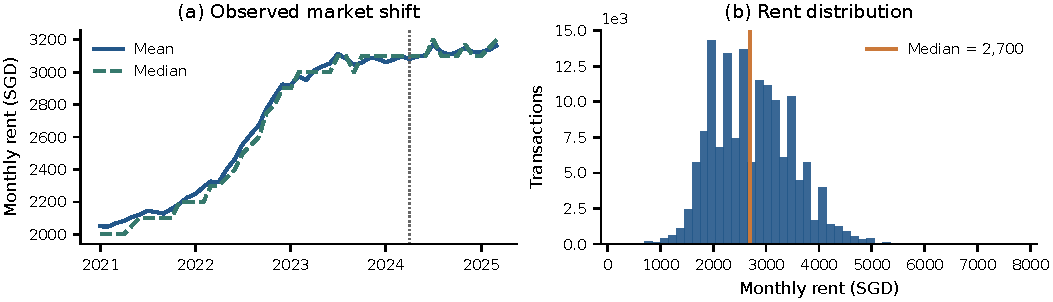
\includegraphics[width=\textwidth]{eda.pdf}
\caption{Training-data EDA. Monthly means and medians show substantial temporal change; the dotted line marks the annual validation start. The marginal distribution spans \sgd300--\sgd7,600. These are descriptive summaries of the supplied training data, not composition-adjusted price indices.}
\label{fig:eda}
\end{figure*}

Raw CSV cells have no missing entries, but semantic cleaning is necessary. There are 425 exact duplicate rows; the principal experiments retain them because the available fields do not identify individual contracts and repetition alone does not establish an error. \code{FURNISHED} and \code{FEE} are constant and are excluded. Flat types contain equivalent spellings such as ``4 room'' and ``4-room''. The naming convention changes strongly with year, so standardizing case, whitespace and separators also removes a formatting proxy for time.

After normalization, the largest groups are 4-room (54,079), 3-room (49,024) and 5-room flats (35,523); only 42 observations are 1-room flats. The median rent is \sgd2,700, the interquartile range is \sgd2,100--\sgd3,200, and the 1st--99th percentile range is \sgd1,300--\sgd4,600. Figure~\ref{fig:eda} motivates explicit calendar and market-history features. Area has a raw Pearson correlation of approximately 0.329 with rent, suggesting that size alone cannot capture temporal and spatial variation. These associations are descriptive and do not establish causal premiums.

\subsection{Auxiliary information and cleaning decisions}
Six supplied auxiliary tables describe HDB blocks, MRT stations, malls, schools, Certificate of Entitlement (COE) premiums and stock prices. The building table has 9,464 entries. Normalized town--block--street keys match all train and test records in the existing auxiliary audit. Postal code ``NIL'' and invalid numeric sentinels such as $-1$ are treated as missing rather than valid values. One training record has a lease commencement year after approval; its negative age proxy is set to missing.

Station records must be deduplicated by physical location: 243 line-level entries represent 192 distinct locations in the supplied audit. Otherwise, interchange stations inflate nearby-station counts. Coordinates support nearest-facility great-circle distance and counts within 1 km. These describe geographical proximity, not measured travel time. Building maximum floor describes building form and must not be interpreted as the rental unit's floor.

The facility tables are static snapshots without complete historical opening dates. We therefore treat them as competition-supplied spatial information, not as fully audited historical inventories. This limits claims about deployable point-in-time accuracy. Similarly, economic series observed after a forecast origin are unavailable in a realistic fixed-origin forecast. Experiments using supplied prediction-month economic observations are explicitly reported as a different information scenario.

Missing numerical history values remain missing for models that support them; counts are zero when a group has no observations. Linear and neural pipelines learn imputation and scaling only on fitting rows. Categorical vocabularies are also learned within each fitting partition, with a reserved unknown category. Neural preprocessing includes categorical embeddings, log-transformed history counts and, where configured, train-fitted numerical transformations. Continuous time retains an extrapolatable linear scale rather than being quantile-clipped at the last observed month.

\subsection{Outliers and duplicate handling}
We do not remove rents merely because they are small or large. A low rent may reflect a valid contract, omitted unit information or a data problem; those explanations cannot be distinguished from the target alone. The main results preserve every validation record. A later training-only half-median filter tests whether removing unusually low rents helps; Section~\ref{sec:errors} reports its deterioration. This makes cleaning a testable modelling decision rather than a way to simplify the evaluation distribution.

\section{Feature Engineering}
\subsection{Static and ordinary historical features}
The compact static representation has 19 inputs: five property variables, three calendar variables, five location variables and six amenity variables. Property inputs include normalized type and model, floor area, age proxy and building maximum floor. Calendar inputs are month index and annual sine/cosine terms. Location inputs include town, planning area, latitude, longitude and distance to the chosen CBD reference point. Each amenity family contributes nearest distance and count within 1 km.

Eight history fields extend this to 27 inputs. At both block $\times$ flat-type and planning-area $\times$ flat-type levels, we calculate expanding mean rent, observation count, latest observed monthly mean and months since the latest observation. For a fitting record in month $t$, these statistics use only months earlier than $t$. For a validation record, the source pool is frozen before the forecast origin $T_0$:
\begin{equation}
\mathcal{H}_i=\{j:g_j=g_i,\ t_j<\min(t_i,T_0)\},
\label{eq:history}
\end{equation}
where $g$ denotes the relevant group. No validation rent updates the pool. For fitting records, $t_i<T_0$, so Equation~\ref{eq:history} reduces to a strictly earlier-month lookup.

This representation supplies both a local price estimate and its reliability. Counts distinguish sparse estimates from well-supported averages; recency distinguishes stale and current information. Unknown block groups can fall back indirectly to area-level information through the model. Four signature-history columns were removed from an earlier 31-column representation after a rowwise audit showed that they duplicated block/type histories in this dataset.

\subsection{Market-relative and anniversary histories}
To separate a location's price level from the national market at the source date, we normalize a historical rent by its source-month flat-type mean:
\begin{equation}
q_j=\frac{y_j}{\overline y_{f_j,t_j}}.
\end{equation}
Twenty summaries over five grouping granularities extend the 27-column representation to 47 columns. Because normalization uses historical source-month rents, it does not require a target-month market mean at inference.

Anniversary features then retrieve same-block, same-flat-type observations around $t_i-L$, for $L\in\{12,24,36\}$ months, with a $\pm1$-month window. Each lag contributes five quantities: sample count, mean rent, mean market ratio, standard deviation of the ratio and fraction with ratio below 0.65. The resulting nested representation has 62 columns. Exact-month and broader-cohort variants are also used by ensemble members. All retrieved records must lie in the fitting pool; unavailable cohorts remain missing with zero support.

The hypothesis is that cohort-specific historical levels preserve information diluted by an expanding average. They might partly reflect recurring rental patterns, but no unit or tenant identifier is available. We therefore do not claim to identify renewals. At long horizons, an anniversary month can lie beyond the frozen source pool; a correct implementation leaves that cohort unavailable.

\subsection{Local temporal baselines and residual targets}
Some enhanced models learn residual rent relative to a baseline $b_i$ built exclusively from earlier information:
\begin{equation}
r_i=y_i-b_i,\qquad \widehat y_i=b_i+\widehat r_i.
\label{eq:residual}
\end{equation}
The baseline is added exactly once before comparing models or blending predictions in SGD. The submitted Transformer branch uses an adjusted historical baseline. The separate aligned TabPFN branch pools flat-type trends and shrunken planning-area premiums, selecting damping and decay using earlier rolling forecasts.

For TabPFN, history features and the temporal baseline share the same simulated origin for each context task. This prevents a training mismatch in which stale forecasts are paired with fresher local histories. Context tasks cover the one-to-ten-month horizons used in recent validation. The TabPFN 77-input representation is a separate feature system; its count must not be interpreted as another step in the 19/27/47/62 ladder.

\section{Methods and Experimental Protocol}
\subsection{Chronological evaluation and comparison scope}
The main annual window is April 2024--March 2025: 114,842 fitting rows precede 35,158 validation rows. The recent window is June 2024--March 2025: 121,005 fitting rows precede 28,995 validation rows. These windows overlap and cannot be counted as independent replications. A 16-month December 2023--March 2025 stress window, and earlier chronological windows, are used in selected studies; stress-window errors are kept separate from annual pooled results.

For the common-input model comparison, October 2023--March 2024 is the inner selection period. Candidate hyperparameters and stopping rounds are chosen there; the selected configuration is refitted on all pre-April rows for a fixed number of rounds. Outer labels do not drive early stopping. This follows the forecasting principle that evaluation targets must occur after the information used to construct their forecasts~\cite{forecasting}. Later blend experiments have their own chronological meta-training cutoffs, described below.

We distinguish three questions. The \emph{common-input comparison} fixes the 27 source features and fitting/validation rows. The \emph{feature ladder} fixes each model's parameters and rounds while adding nested feature groups. The \emph{pipeline comparison} allows enhanced representations and blending. Differences between pipelines cannot be attributed solely to architecture.

The primary metric is original-scale root mean squared error:
\begin{equation}
\operatorname{RMSE}=\sqrt{\frac{1}{n}\sum_{i=1}^{n}(\widehat y_i-y_i)^2}.
\end{equation}
We also report mean absolute error (MAE) and mean signed bias, $n^{-1}\sum_i(\widehat y_i-y_i)$. Positive bias means overprediction. Where disjoint folds are pooled, their summed squared errors and row counts are pooled before taking the square root; fold RMSEs are not averaged directly.

\subsection{Model families and tuning}
Ridge regression provides a linear reference, with $\alpha\in\{1,100,10000\}$ selected on the inner window. ExtraTrees tests randomized bagging. LightGBM~\cite{lightgbm}, XGBoost~\cite{xgboost} and CatBoost~\cite{catboost} test strong nonlinear tabular baselines with different handling of sparse and categorical inputs. Embedding MLP and FT-Transformer~\cite{ft} test whether learned category representations and feature attention improve on trees.

The archived search uses a limited candidate set rather than exhaustive tuning: LightGBM tests 31/63 leaves, CatBoost depth 6/8, and XGBoost depth 4/6, alongside representation variants. Common-input comparisons restrict eligibility to the compact profile. Inner-selected training lengths are 108 LightGBM trees, 448 XGBoost rounds, 814 CatBoost rounds, 300 ExtraTrees trees, 29 MLP epochs and five FT-Transformer epochs. The MLP uses width 256 and learning rate $10^{-3}$; the compact FT uses width 96 and learning rate $3\!\times\!10^{-4}$. Search budgets and preprocessing differ across families, so the comparison is controlled for information rather than total compute.

The feature ladder has a separate, fixed configuration: LightGBM uses 353 trees, 15 leaves, learning rate 0.03 and L2 penalty 10; CatBoost uses 535 iterations, depth 6, learning rate 0.04 and L2 penalty 10. These settings stay constant across all four feature levels within each model. Their 27-input errors therefore need not equal those of the separately tuned common-input models.

\subsection{Numerical embeddings and structural alternatives}
The enhanced Transformer study compares linear numerical tokens, piecewise-linear embeddings (PLE), and learnable periodic embeddings (PLR)~\cite{numembed}. The selected PLR-FT member has width 128, three attention blocks, eight heads and learning rate $10^{-4}$. It uses 16 periodic frequencies per numerical feature. Training uses AdamW with weight decay 0.001; the earlier-window epoch cap is 16 with patience four. Later refits use the selected epoch count without validation stopping.

New neural members omit five sparse 36-month cohort statistics and learn residuals relative to the adjusted history baseline. A four-seed average of the pruned FT is one ensemble channel. Additional bounded-budget alternatives include a DCN-V2-style full-matrix cross network~\cite{dcn}, soft-gated expert networks and asymmetric CatBoost trees. These are project adaptations, not claims of reproducing published benchmark results. Their negative and mixed results inform the final selection.

\subsection{Regularized blending conditioned on history coverage}
The archived final pipeline contains 12 prediction channels: seven historical tree members, two XGBoost members, the original FT, a four-seed pruned-FT average and a PLR-FT member. Thus it contains 15 trained predictors, not 15 architectures. All outputs are first reconstructed as SGD rents.

Let $e_{ik}=(p_{ik}-y_i)/1000$ be model $k$'s historical out-of-time error. For blend fitting, each model's within-month weighted mean error is subtracted to obtain $\widetilde e_{ik}$. Global weights solve
\begin{equation}
\begin{aligned}
\min_w\quad &\sum_i a_i(\widetilde e_i^{\mathsf T}w)^2+
\lambda\|w-w^{(0)}\|_2^2,\\
\text{subject to}\quad &\mathbf{1}^{\mathsf T}w=1,\quad 0\leq w_k\leq0.6,
\end{aligned}
\label{eq:blend}
\end{equation}
with $\lambda=0.003$ and prior $w^{(0)}$ from the preceding ensemble. Dividing errors by 1,000 is part of the penalty's scale. Month-centering aims to reduce sensitivity to historical market-level bias. It is used only during weight estimation; inference directly averages predictions and never needs a query-month error mean.

The presence or absence of 24- and 36-month cohort support defines at most four groups. Group weights solve the same problem with the global solution as prior and penalty 0.003. Groups with fewer than 500 meta-training observations, and unseen groups, use global weights. Annual blend labels stop at March 2024; recent weights may include April--May out-of-time predictions made by pre-April models. The final full-data blend uses 53,135 historical out-of-time predictions from October 2023--March 2024 and April 2024--March 2025, weighting the two forecast-origin pools equally.

The month-centered grouping recipe and the decision to include PLR were selected after examining later development results. Chronological weight fitting prevents direct use of a query's label in its own forecast, but does not erase this adaptive model-selection bias.

\section{Evaluation and Interpretation}
\subsection{Common-input models}
\begin{table}[t]
\caption{Common 27 inputs; 35,158 annual validation rows. All errors are in SGD. Bias is prediction minus actual rent.}
\label{tab:models}
\centering\small
\begin{tabular}{lrrr}
\toprule
Model & RMSE & MAE & Bias \\
\midrule
Ridge & 513.03 & 363.23 & +194.11 \\
ExtraTrees & 468.47 & 341.08 & +4.79 \\
LightGBM & 468.87 & 340.71 & +11.67 \\
XGBoost & 467.03 & 338.87 & +20.64 \\
CatBoost & 468.46 & 343.51 & -3.71 \\
Embedding MLP & 483.72 & 358.21 & -11.83 \\
FT-Transformer & 476.00 & 339.92 & +87.64 \\
\bottomrule
\end{tabular}

\end{table}

Table~\ref{tab:models} shows that the tested tree models outperform the tested MLP and FT configurations on annual RMSE. XGBoost has the smallest error, \sgd467.03, compared with \sgd513.03 for Ridge and \sgd476.00 for FT. The training-mean benchmark is much worse at \sgd846.75. Nonlinear models therefore offer a substantial improvement over these simple references.

However, differences among the tree methods are small: the XGBoost--LightGBM gap is only \sgd1.84. The archived three-month-block sensitivity interval for this gap is approximately $[-2.48,-1.28]$, conditional on the saved predictions. This is not an architecture-wide superiority claim. Single seeds, unequal search budgets and reuse of the annual period limit that interpretation.

FT's MAE of \sgd339.92 is close to the strongest trees despite a larger RMSE and positive bias. This suggests that its error distribution differs from theirs and motivates checking complementarity, but a different bias or lower error correlation alone does not guarantee that adding it improves a blend.

\subsection{Controlled feature contributions}
\begin{figure*}[t]
\centering
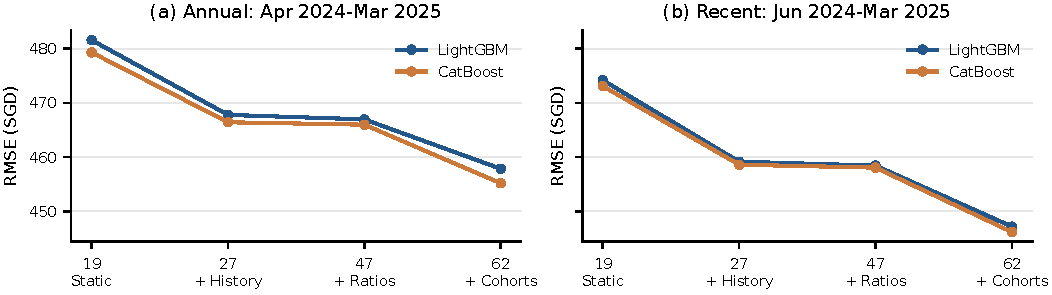
\includegraphics[width=\textwidth]{feature_ladder.pdf}
\caption{Controlled nested feature ladder. Parameters, training rounds and evaluation rows are fixed within each model/window. Ordinary histories and anniversary cohorts provide clearer gains than the intermediate market-ratio expansion. Annual and recent windows overlap.}
\label{fig:ladder}
\end{figure*}

\begin{table}[t]
\caption{Feature ladder RMSE (SGD). Counts denote nested input sets, not changes of model architecture.}
\label{tab:ladder}
\centering\small
\begin{tabular}{lrrrr}
\toprule
Model / window & 19 & 27 & 47 & 62 \\
\midrule
LightGBM / annual & 481.60 & 467.80 & 466.97 & 457.84 \\
LightGBM / recent & 474.18 & 459.15 & 458.43 & 447.17 \\
CatBoost / annual & 479.33 & 466.43 & 465.99 & 455.17 \\
CatBoost / recent & 473.11 & 458.60 & 458.06 & 446.16 \\
\bottomrule
\end{tabular}

\end{table}

The fixed-model ladder in Table~\ref{tab:ladder} and Figure~\ref{fig:ladder} supports two clear gains. Adding ordinary histories reduces annual LightGBM RMSE by \sgd13.81, from 481.60 to 467.80. Adding anniversary cohorts to the 47-input model reduces it by another \sgd9.12, to 457.84. CatBoost shows the same direction, ending at 455.17. Market-relative histories alone yield smaller increments: approximately \sgd0.83 for annual LightGBM and \sgd0.45 for annual CatBoost.

Group-deletion experiments provide a complementary check. On the compact 27-input LightGBM model, removing all history fields raises pooled three-annual-window RMSE by \sgd7.94, while removing time and all histories together raises it by \sgd141.33. Removing all amenity fields raises pooled error by only \sgd0.58, with inconsistent window-level effects. Predictors can substitute for one another, so single-column deletions are not additive importance shares. Retained histories may still encode location or flat type when direct location/type inputs are removed.

The small conditional amenity gain does not establish that amenities are economically unimportant. Location and past rents may already absorb much of their predictive information, and static facility snapshots are imperfect proxies. The evidence supports prioritizing time and history engineering under this evaluation design.

Supplementary Figure~\ref{fig:appendixfeatures} visualizes the deletion results and the availability of anniversary histories. In the TabPFN cohort study, 36-month support is available for only 8.5\% of fitting records, compared with 63.2\% of validation records. This support mismatch is a reason to inspect sparse long-lag features carefully, rather than assuming more history always improves transfer.

\subsection{Enhanced pipeline validation and structural ablations}
\begin{table*}[t]
\caption{Enhanced pipeline validation in SGD. Annual: April 2024--March 2025, 35,158 rows. Recent: June 2024--March 2025, 28,995 rows. These development windows overlap and have been reused during model selection.}
\label{tab:final}
\centering\small
\begin{tabular}{lrr}
\toprule
Pipeline & Annual RMSE & Recent RMSE \\
\midrule
History ensemble & 451.1810 & 442.9025 \\
Tree/Transformer + PLR-FT & 451.0295 & 441.8345 \\
Trees + TabPFN, original categories & -- & 440.9520 \\
Trees + TabPFN, grouped flat models & -- & \textbf{440.7707} \\
\bottomrule
\end{tabular}

\end{table*}

Among the three archived pipelines in Table~\ref{tab:final}, the grouped tree/Transformer ensemble with PLR-FT has the lowest annual and recent validation RMSE. Relative to the history ensemble, annual RMSE falls from 451.1810 to 451.0295 and recent RMSE from 442.9025 to 441.8345. These differences are small, particularly on the annual window, and reflect complete pipelines rather than an isolated architecture change. The later TabPFN comparisons below provide additional recent-window evidence without establishing superiority across all forecast origins.

The macro-enhanced variant uses a different information scenario, including supplied prediction-month economic observations. It changes recent local RMSE by only \sgd0.0133 relative to the historical baseline and slightly worsens annual RMSE. It is not part of the grouped structure ensemble and does not justify assuming that future economic data will be available in deployment.

The final-versus-history gain combines several changes: history pruning, seed averaging, conditional blending and PLR output. It cannot all be credited to PLR. Holding the grouped-blending rule fixed, adding only PLR changes recent RMSE from 441.9591 to 441.8345, but worsens annual RMSE from 450.8650 to 451.0295. The improvement is therefore not uniform across origins.

PLR-FT is also not the best standalone network: PLE-FT records annual/recent errors of 458.29/449.82, versus 462.07/451.10 for PLR-FT. PLR's value is conditional complementarity within this blend. Adding every new architecture instead yields recent RMSE 442.51, worse than the grouped baseline. Increased model count does not guarantee useful diversity, and bounded weight optimization can still overfit historical error patterns.

\subsection{Separate TabPFN follow-up}
\begin{table}[t]
\caption{Separate recent-window follow-up: frozen TabPFN-3.5-Fast and the reproduced seven-tree ensemble. This tree ensemble is an earlier model, not the submitted 12-channel final.}
\label{tab:tabpfn}
\centering\small
\begin{tabular}{llrr}
\toprule
Model & Inputs & RMSE & MAE \\
\midrule
Frozen Fast control & 77 & 455.396 & 327.794 \\
+ 12/24-month cohorts & 87 & 441.959 & 318.216 \\
+ 12/24/36-month cohorts & 92 & 442.016 & 317.815 \\
Seven-tree ensemble & varied & 443.863 & 322.919 \\
Earlier-locked blend & varied & 442.302 & 321.032 \\
Equal blend & varied & 440.952 & 318.888 \\
\bottomrule
\end{tabular}

\end{table}

The foundation-model branch uses TabPFN-3.5-Fast~\cite{tabpfn35}, full 121,005-row context, seed 42 and two internal estimator views. In a matched ablation, its original 77 inputs, residual target, temporal baseline and checkpoint stay fixed. Adding ten 12/24-month cohort inputs reduces RMSE from 455.396 to 441.959 (Table~\ref{tab:tabpfn}), a \sgd13.437 gain. Five additional 36-month fields yield 442.016, providing no further observed RMSE improvement.

Combining the 87-input TabPFN with the reproduced seven-tree ensemble at equal weights yields 440.952. A TabPFN weight of 0.1893 fitted on October 2023--March 2024 forecasts instead yields 442.302 on the recent window. Thus the attractive equal-blend result should be read alongside the less favorable earlier-locked choice. It improves all ten months relative to TabPFN and nine relative to the tree ensemble, but the same months have already informed multiple experiments.

Replacing direct flat-model categories with a proposed coarser grouping yields a further small blend decrease to 440.771, but its descriptive month-cluster interval includes no improvement and errors worsen among the 126 validation rows whose labels change. This is insufficient to establish a robust grouping benefit. We therefore emphasize the matched cohort ablation and the ungrouped equal-blend result, while retaining the coarser-group result as a sensitivity analysis requiring confirmation at other chronological origins.

\subsection{Error patterns and training-only cleaning}\label{sec:errors}
\begin{figure*}[t]
\centering
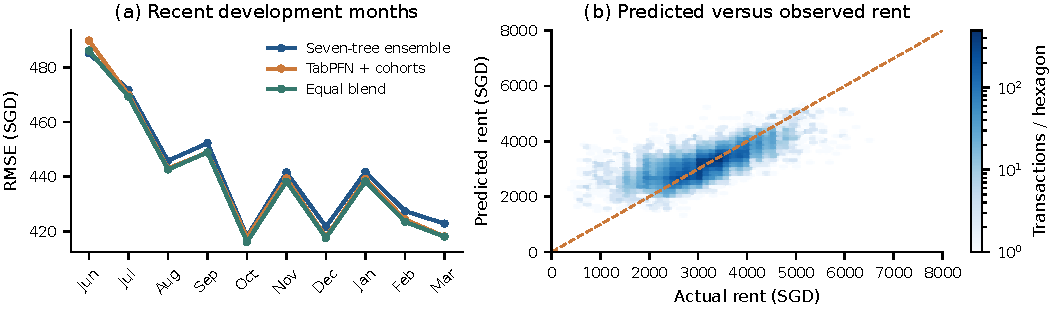
\includegraphics[width=\textwidth]{error_analysis.pdf}
\caption{Diagnostics for the separate equal tree/TabPFN blend, not the archived submitted ensemble. Left: performance varies by month and market regime. Right: log-density hexagons show regression toward central rents, with substantial overprediction of some low-rent records. The dashed line is perfect prediction.}
\label{fig:errors}
\end{figure*}

Figure~\ref{fig:errors} shows that error varies by month and by rent level. For this same equal tree/TabPFN blend, 1,643 validation records (5.7\%) have actual rent at most \sgd2,000, yet account for 32.8\% of squared error. Their RMSE is \sgd1,061.54 with positive bias \sgd935.91. Among 1,998 records above \sgd4,000, RMSE is \sgd607.08 and bias is negative \sgd466.52. Supplementary Figure~\ref{fig:appendixerrors} compares these groups' sample and error shares. These are post-hoc target groups; true rent must not be used to choose a correction at inference.

The later half-median ablation removes fitting rents below half their year $\times$ town $\times$ normalized-flat-type median, computed only within the fitting partition. It removes 848 of 121,005 fitting rows and rebuilds all affected histories, market normalizers and temporal baselines. Validation remains all 28,995 original rows, and model hyperparameters and blend weights stay fixed.

\begin{table}[t]
\caption{Training-only outlier-filter ablation on the separate equal tree/TabPFN blend. Validation is unchanged. Errors are in SGD.}
\label{tab:filter}
\centering\small
\begin{tabular}{lrrr}
\toprule
Model & RMSE & MAE & Bias \\
\midrule
All fitting rows & 440.95 & 318.89 & -0.40 \\
Half-median filter & 445.84 & 316.56 & 32.77 \\
\bottomrule
\end{tabular}

\end{table}

Filtering increases RMSE by \sgd4.89 and improves only one of ten months (Table~\ref{tab:filter}). MAE falls slightly, but positive bias rises to \sgd32.77. Of the supported validation groups, 189 records lie below the training-derived cutoff; their unfiltered RMSE is \sgd1,751.04 and rises to \sgd1,860.71 after filtering. The filter improves neither the primary objective nor the difficult tail. The 2025 rows lack a same-year fitting cutoff, illustrating another limitation of this retrospective rule.

These results show why removing statistical outliers is not equivalent to repairing verified label errors. The target contains meaningful heterogeneity that the observed inputs may not explain. More useful next steps are auditing source reliability, adding permissible unit-level information, and modelling uncertainty rather than automatically discarding low rents.

\section{Limitations and Reproducibility}
\subsection{What the evaluation supports}
All reported development periods have been examined repeatedly. Earlier-only features, train-fitted preprocessing and chronological weight cutoffs prevent important forms of direct leakage, but do not create an untouched final test after extensive adaptive search. Some selected blends were explicitly chosen after inspecting later errors. The displayed Kaggle comparison also informed the archived final selection. Small gains should be treated as development evidence rather than confirmatory significance.

Archived uncertainty analyses resample paired errors by months or contiguous month blocks, retaining rentals within each sampled time unit. These recognize shared shocks better than independent-row bootstrap. Nevertheless, ten or twelve months provide limited temporal support; fixed-prediction intervals omit training, selection and future-regime uncertainty. They should not be presented as strong generalization guarantees.

For the recent matched comparisons, Appendix~B reports a uniform paired three-month-block sensitivity analysis. It preserves candidate/reference alignment and recomputes pooled RMSE within each resample. Month-by-month errors at a single origin confound forecast horizon with calendar conditions; they cannot separately identify the effect of increasing horizon.

The test spans 17 calendar months and includes horizons longer than the ten-month recent validation. In the full-data TabPFN policy, 18,077 test records lie beyond that validated range; the inherited temporal level and uncertainty plateau at month ten. This is a pragmatic extrapolation policy, not evidence of accuracy at those horizons. The archived 16-month stress tests cover only selected earlier pipelines and cannot validate every final configuration.

Final competition refits use all 150,000 supplied labels, including March 2025, while test records also start in March. This follows the available labelled-context setup, but is not equivalent to forecasting every test record from a strict pre-March deployment origin. Lagged rental-feature cutoffs and the labels supplied to the fitted model are distinct information boundaries. A deployment evaluation should fix a common origin and exclude all labels unavailable then.

\balance
\subsection{Reproduction and remaining evidence gaps}
The repository separates preprocessing, feature generation, evaluation and experiment runners, with a core environment specification and optional model dependencies. Source hashes, row IDs, feature schemas, chosen iterations, predictions and blend weights are recorded by the existing workflows. Regression tests cover temporal boundaries, reconstruction, alignment and blending constraints. The workload appendix and source notes support navigation without carrying essential methodological explanation outside the main text.

For this report, a deterministic figure/table builder rechecks raw split sizes, duplicate count, saved prediction IDs, months and labels. It independently reconstructs the recent tree/TabPFN metrics and the unfiltered control. The archived final-structure and Kaggle numbers are read from the retained selection record; the original screenshot and root \code{output/} model artifacts are not present in this checkout. We therefore do not claim to have replayed the complete submitted model during report preparation. Restoring those artifacts or retraining the dependency chain is necessary for an end-to-end submission replay.

\section{Conclusion}
Time-bounded rental histories are the most consistent source of predictive improvement in this study. Controlled comparisons show that tested tree models are strong with common inputs, while ordinary and anniversary histories improve both LightGBM and CatBoost. Conditional blending and numerical embeddings provide smaller, mixed increments rather than a universal architectural advantage. The grouped tree/Transformer pipeline reaches annual/recent validation RMSE of 451.03/441.83; the separate equal tree/TabPFN blend reaches 440.95 on the recent window. These are development results, and additional chronological origins are needed to assess transfer. Future work should prioritize an untouched evaluation, validated longer horizons, source-quality audits and permissible unit-level attributes before expanding the model search.

\clearpage
\nobalance
\begin{thebibliography}{10}
\bibitem{housing} T. F. Sing, J. J. Yang, and S. M. Yu, ``Boosted tree ensembles for artificial intelligence based automated valuation models (AI-AVM),'' \emph{The Journal of Real Estate Finance and Economics}, vol. 65, no. 4, pp. 649--674, 2022. doi: 10.1007/s11146-021-09861-1.
\bibitem{treebenchmark} L. Grinsztajn, E. Oyallon, and G. Varoquaux, ``Why do tree-based models still outperform deep learning on typical tabular data?'' in \emph{Advances in Neural Information Processing Systems}, vol. 35, 2022. [Online]. Available: \url{https://arxiv.org/abs/2207.08815}
\bibitem{forecasting} R. J. Hyndman and G. Athanasopoulos, \emph{Forecasting: Principles and Practice}, 3rd ed. Melbourne, Australia: OTexts, 2021, sec. 5.10. [Online]. Available: \url{https://otexts.com/fpp3/toolbox.html#time-series-cross-validation}
\bibitem{lightgbm} G. Ke \emph{et al.}, ``LightGBM: A highly efficient gradient boosting decision tree,'' in \emph{Advances in Neural Information Processing Systems}, vol. 30, 2017. [Online]. Available: \url{https://proceedings.neurips.cc/paper/2017/hash/6449f44a102fde848669bdd9eb6b76fa-Abstract.html}
\bibitem{xgboost} T. Chen and C. Guestrin, ``XGBoost: A scalable tree boosting system,'' in \emph{Proc. ACM SIGKDD}, 2016, pp. 785--794. doi: 10.1145/2939672.2939785.
\bibitem{catboost} L. Prokhorenkova, G. Gusev, A. Vorobev, A. V. Dorogush, and A. Gulin, ``CatBoost: Unbiased boosting with categorical features,'' in \emph{Advances in Neural Information Processing Systems}, vol. 31, 2018. [Online]. Available: \url{https://arxiv.org/abs/1706.09516}
\bibitem{ft} Y. Gorishniy, I. Rubachev, V. Khrulkov, and A. Babenko, ``Revisiting deep learning models for tabular data,'' in \emph{Advances in Neural Information Processing Systems}, vol. 34, 2021. [Online]. Available: \url{https://arxiv.org/abs/2106.11959}
\bibitem{numembed} Y. Gorishniy, I. Rubachev, and A. Babenko, ``On embeddings for numerical features in tabular deep learning,'' in \emph{Advances in Neural Information Processing Systems}, vol. 35, 2022. [Online]. Available: \url{https://arxiv.org/abs/2203.05556}
\bibitem{dcn} R. Wang \emph{et al.}, ``DCN V2: Improved Deep \& Cross Network and practical lessons for web-scale learning to rank systems,'' in \emph{Proc. The Web Conference}, 2021. doi: 10.1145/3442381.3450078.
\bibitem{tabpfn35} B. J\"ager \emph{et al.}, ``TabPFN-3.5: Technical report,'' arXiv:2609.17895, 2026. [Online]. Available: \url{https://arxiv.org/abs/2609.17895}
\end{thebibliography}

\clearpage
\appendices
\section{Team Workload and Reproduction Notes}
\begingroup\raggedright
\noindent\textbf{Team details are placeholders.} Insert the confirmed team name, every member's name and student ID in the author block, and replace the ownership entries below with the actual division of work. The table lists project activities; it does not assert who performed them or invent contribution percentages.

\begin{table}[h]
\caption{Workload breakdown to be completed by the team. Multiple members may share an activity.}
\centering\small
\begin{tabular}{p{.52\columnwidth}p{.36\columnwidth}}
\toprule
Activity & Member(s), student ID(s)\\
\midrule
EDA, source checks and preprocessing & To be supplied\\
Spatial and rental-history features & To be supplied\\
Tree models and chronological evaluation & To be supplied\\
Transformer / TabPFN experiments & To be supplied\\
Ensembling and submission verification & To be supplied\\
Report, visualizations and reproducibility & To be supplied\\
\bottomrule
\end{tabular}
\end{table}

\subsection{Supplementary competition record}
Validation results are the primary evidence in this report. For completeness, the archived November 5, 2026 selection record lists Kaggle displayed scores of 415.86912 for the history ensemble, 415.78232 for the macro variant, and 415.37529 for the grouped ensemble with PLR-FT. Its source screenshot is unavailable here and does not identify the public/private partition. These figures are supplementary archival context, not independently verified test results or a replacement for the chronological comparisons.

\subsection{Evidence locations}
Paths below are relative to the repository root. Model scores in the paper are local project results; method references describe algorithms rather than supplying those scores.
\begin{itemize}
\item Data audit: \path{reports/train_test_eda/summary.json} and \path{reports/auxiliary_data_eda/summary.json}.
\item Common inputs: \path{experiment/03_model_comparison/same_input_models.csv} and \path{recommended_models.csv} in the same directory.
\item Feature ladder: \path{experiment/02_feature_engineering/controlled_feature_ladder.csv}; group deletions: \path{group_feature_effects.csv} in the same directory.
\item Submitted pipeline and Kaggle provenance: \path{experiment/01_final/submission_selection.json}. The recorded screenshot source was not available for fresh visual verification.
\item Grouped blending and PLR comparisons: \path{experiment/04_optimization_history/09_grouped_blending.md} and \path{10_plr_transformer_final.md} in the same directory.
\item Matched TabPFN cohort study: \path{reports/tabpfn_anniversary_history_80_20/}; tree/TabPFN comparison: \path{reports/zch_anniversary_tabpfn_blend/}.
\item Cleaning and category grouping: \path{reports/half_median_zch_tabpfn_ensemble/} and \path{reports/flat_model_grouping_ensemble/}.
\end{itemize}

\subsection{Practical reproduction sequence}
Create the core environment from \path{environment.yml}. Use \path{docs/guides/running_experiments.md} for the dependency order; later rounds reuse earlier trained predictors and out-of-time predictions. The preflight command
\begin{quote}\small\ttfamily
python -m analysis.main preflight --profile final
\end{quote}
checks required final-model resources without training. Missing ignored model artifacts must be restored or rebuilt; running only the final blending script is insufficient.

The common-input comparison is exposed through \code{analysis.main common-models}. The controlled ladder is exposed through \code{analysis.experiments.report\_selection\_trials ladder}, separately for \code{--stage outer} and \code{--stage june}. The anniversary and cleaning follow-ups have dedicated scripts \path{analysis/compare_tabpfn_anniversary_history_80_20.py}, \path{analysis/compare_zch_anniversary_tabpfn_ensemble.py}, and \path{analysis/compare_half_median_ensemble.py}.

The paper's tables, plots and evidence hashes are regenerated without model fitting by
\begin{quote}\footnotesize\ttfamily
python reports/final\_report/build\_report.py
\end{quote}
Compile \path{reports/final_report/final_report.tex} using an IEEEtran-capable LaTeX installation. The report build audit distinguishes recomputed recent prediction metrics from archived final-selection values. This manuscript does not contain any measured score for unlabelled test rows beyond the saved Kaggle displayed comparison.

\par\endgroup

\clearpage
\onecolumn
\section{Supplementary Validation Diagnostics}
These supplementary results retain the main text's information boundaries. No additional model is fitted, and all recent-window comparisons use the same 28,995 original validation rows.

\begin{figure}[!ht]
\centering
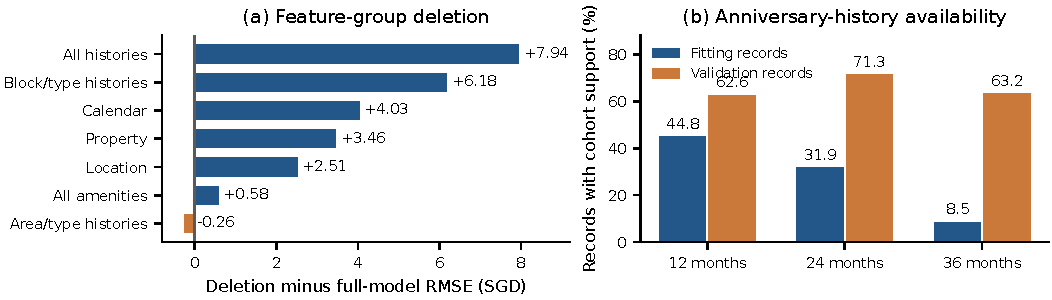
\includegraphics[width=\textwidth]{appendix_feature_diagnostics.pdf}
\caption{Feature evidence. Left: fixed 27-input LightGBM group deletions, pooled over the three annual windows from April 2022--March 2025. Positive differences mean removal worsens RMSE; groups overlap and effects are not additive. The joint time-plus-history deletion, omitted from this scale, increases error by \sgd141.33. Right: cohort support in the separate TabPFN study (121,005 fitting and 28,995 validation records). Validation histories remain frozen at May 2024. Sparse fitting support and later query support need not match.}
\label{fig:appendixfeatures}
\end{figure}

\begin{figure}[!ht]
\centering
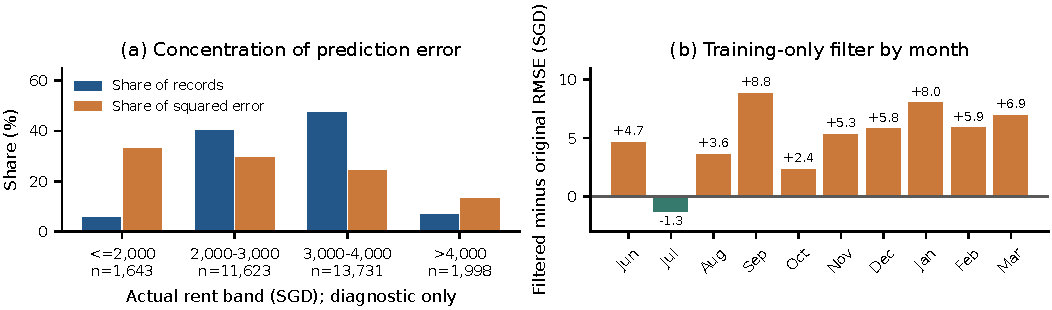
\includegraphics[width=\textwidth]{appendix_error_diagnostics.pdf}
\caption{Error concentration and cleaning sensitivity for the equal seven-tree/87-input TabPFN blend. Left: actual-rent groups are diagnostic only, with upper-inclusive boundaries and sample counts shown. The low-rent tail contributes far more squared error than its sample share. Right: the training-only half-median filter worsens RMSE in nine of ten June 2024--March 2025 months. All validation rows remain included. A single origin confounds horizon with calendar month.}
\label{fig:appendixerrors}
\end{figure}

\begin{table}[!ht]
\caption{Paired recent-window RMSE sensitivity (SGD); negative values favor the first candidate. Input counts follow Table~\ref{tab:tabpfn}. Intervals use 5,000 circular three-month-block resamples of ten months, seed 42. Sampled months retain all their rows; pooled squared errors and counts determine each RMSE.}
\label{tab:paired}
\centering\small
\begin{tabular}{lrrr}
\toprule
Contrast & $\Delta$RMSE & 95\% block interval & Months improved \\
\midrule
87 vs 77 inputs & -13.437 & [-16.273, -10.991] & 10/10 \\
92 vs 87 inputs & +0.057 & [-0.542, +0.773] & 4/10 \\
Equal blend vs 87 & -1.007 & [-1.527, -0.567] & 10/10 \\
Earlier-locked blend vs 87 & +0.343 & [-0.656, +1.156] & 2/10 \\
Coarser categories vs original & -0.181 & [-0.499, +0.143] & 6/10 \\
Half-median filter vs original & +4.891 & [+3.170, +6.461] & 1/10 \\
\bottomrule
\end{tabular}

\end{table}

\noindent The cohort gain is consistent across months; coarser-category and 36-month additions remain uncertain. These descriptive intervals condition on fixed predictions and omit model-fitting and adaptive-selection uncertainty. Ten reused months provide limited temporal support and do not constitute an independent test.
\end{document}
